\section{Bladder Cancer}


% Overview of the bladder cancer stats
According to Cancer Research UK, bladder cancer is the 10th most common cause of cancer and the 11th most common cancer in the UK \cite{Cancer_Research_UK2015-cf}. This is equivalent to $\sim10,000$ cases from which  $\sim5000$ are deaths, with a 5-year survival rate of 52.6\%. In 2008\cite{Ferlay2010-sx} the worldwide estimates for bladder cancer was $\sim380,000$ new cases and $\sim150,000 $deaths per year. In 2020\cite{Sung2021-hn} , there were $\sim573,000$ cases with $\sim212,536$ deaths reported which shows a considerable increase in the cancer cases\footnote{A good resource to get an overview of the prevelance of bladder cancer (and other cancers too) is the website from World Health Organisation, particularly the trends in cancer overtime: \href{https://gco.iarc.fr/en}.}. Men are 3 times more likely to develop bladder cancer and bladder cancer is specific to Western countries\cite{Knowles2015-mu}. 

% Talk about bladder cancer causes, economical burden
One of the main causes of bladder cancer is caused by smoking, being thought to provoke 50\% of the cases\citet{Knowles2015-mu}. However, the underling biological process on how smoking causes cancer is not understood. Other environment risk factors are metal contamination such as arsenic-water or exposure to ionising radiation\citet{Knowles2015-mu}. 

% Types of bladder 
There are multiple systems to classify bladder depending on their utility. For medical doctors there are two popular systems to dichotomies the bladder cancer Tumour-Node-Metastasis (TNM) and the Internail Sociecty of Urological Pathology (ISUP). The stages of the bladder cancer and the two naming conventions can be seen in \cref{fig:lit:bladder_cancer_stages}; image taken from the bladder cancer review from \citet{Knowles2015-mu}. The figure should be taken as an illustration of the stages and their classification, and not as the evolution of the bladder cancer.

\begin{figure}[!htb]    
    \centering
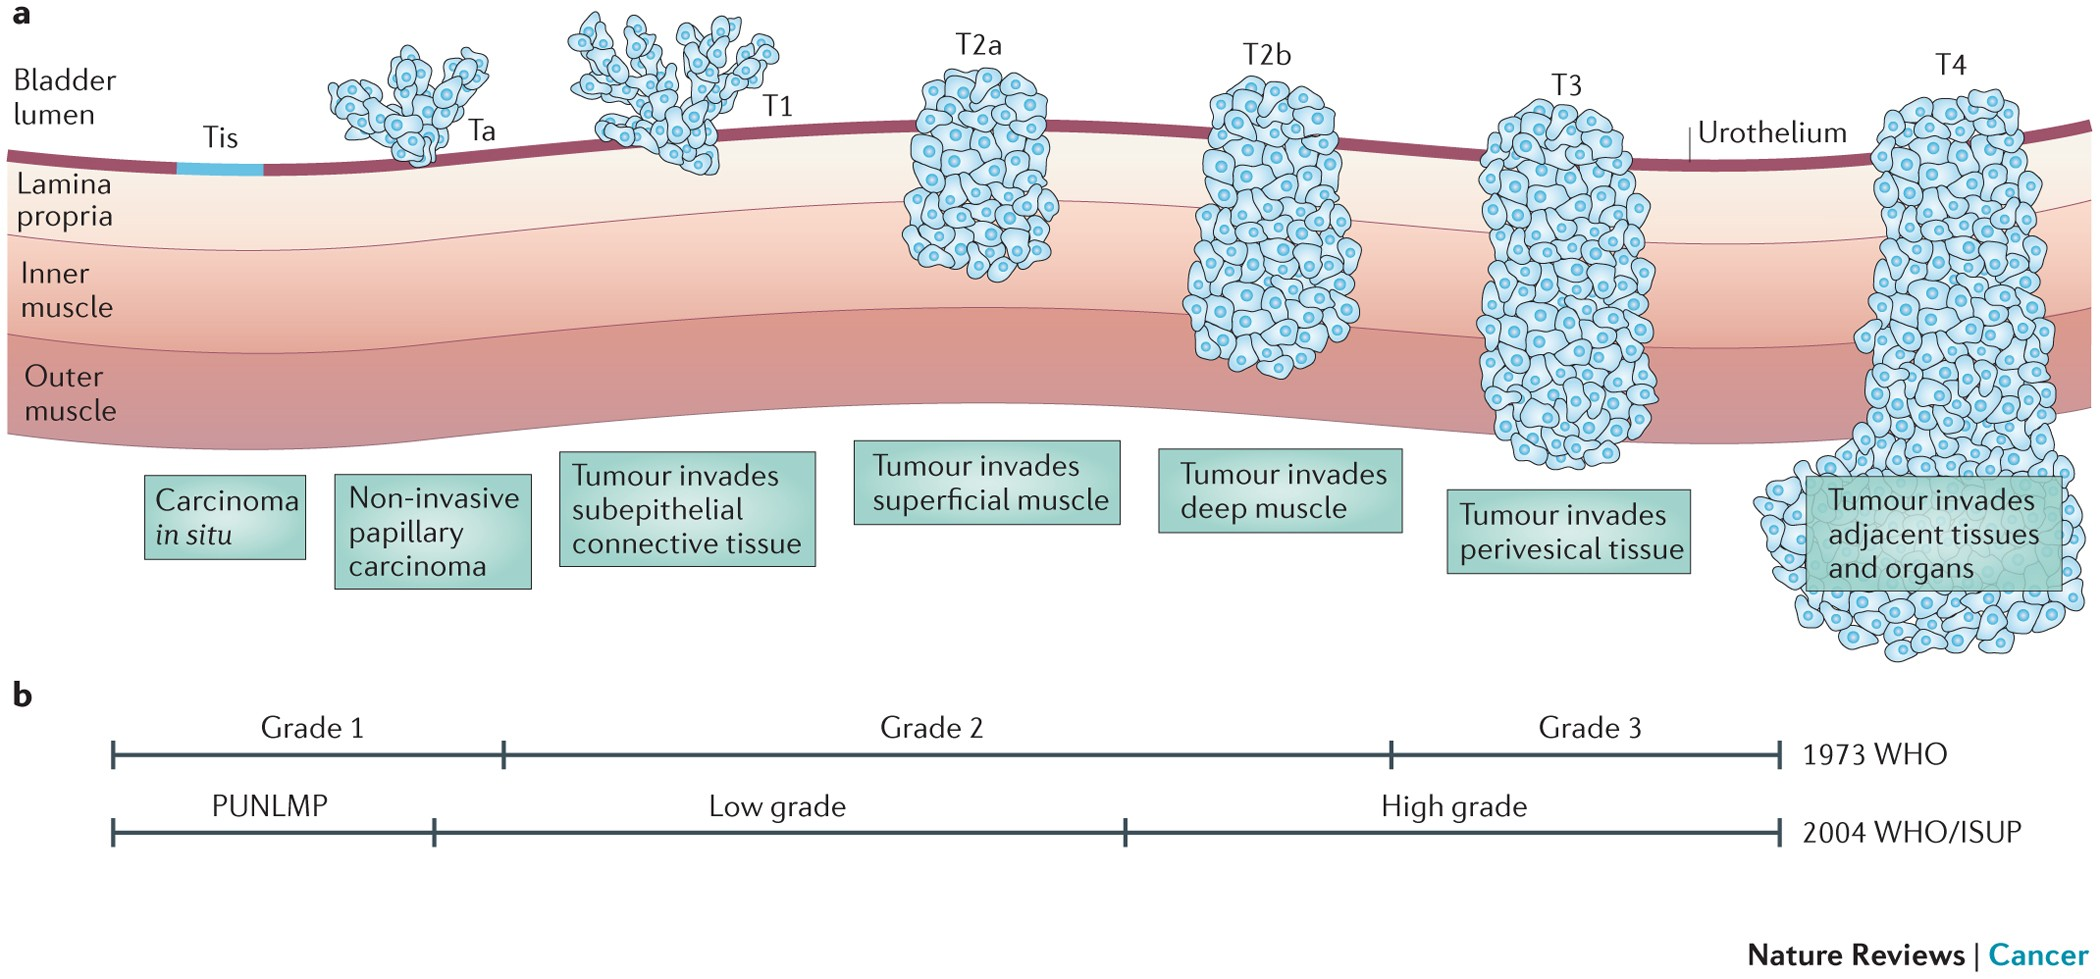
\includegraphics[width=0.9\textwidth,height=0.9\textheight,keepaspectratio]{Sections/Lit_review/Resources/bladder_cancer_grading.jpg}
    \caption{"Bladder cancer grading and staging" from \cite{Knowles2015-mu}. It displays the two grading of the bladder cancer based on its stage. Image a) should be taken just as an illustration of the different stages of bladder cancer and not mistaken with the disease evolution. }
    \label{fig:lit:bladder_cancer_stages}
\end{figure}


There are two main types of bladder cancer: non-muscle invasive (NMIBC) and muscle-invasive bladder cancer (MIBC). From \cref{fig:lit:bladder_cancer_stages} stages Tis, Ta and T1 are classified as NMIBC as they do not invaded the muscle. NMIBC appears in $\sim70\%$ of the bladder patients, it has a high 5-year survival rate with $\sim90\%$, it frequently recurs in 50-70\% of the cases and only 10-15\% progress to muscle invasion\cite{Knowles2015-mu}. Thus, patients suffering from this type of bladder cancer have favourable prognostics but their quality of life is impact as they need to attend periodical cystocopies checkups.

The muscle invasive bladder cancer encompass the T2a, T2b, T3 and T4 stages and it appears in $\sim30\%$ of the bladder cancer cases. It is more aggressive than the NMIBC with $\sim50\%$ 5-year survival prognosis, almost half of the cases of MIBC develop metastasis and for these patients the median survival is 12-15 months\cite{Knowles2015-mu}. 

The patients diagnosed with MIBC undergo cystectomy which removes the entire bladder and has a larger impact to quality of life, while the NIMBC patients have regular cystocopies checkups. Both procedures have a negative impact of the patients and carer's quality of life, and bring an financial burden to them and the healthcare system. Thus, there is a need to develop better diagnosis tools and treatment plants for bladder cancer, especially for the MIBC.

\paragraph*{MIBC subtyping}

% Introduction of TCGA
There are two comprehensive studies of the muscle-invasive bladder cancer (MIBC) cohort from The Cancer Genome Atlas (TCGA) \citet{Tcga2014-dr} and \citet{Robertson2017-mg}. The first is the initial research analysing the fist batch of patient samples (131) while the other analysed the entire cohort of 412 patient samples. The MIBC cohort from TCGA is an invaluable asset for the research community as a number of sequencing techniques were applied to the samples: mRNAseq (gene expression), WEX and WGS (somatic mutations), microarray-based (copy number variations) as well as metadata about the patients. This cohort is characterised by aggressive tumours, having a high grade muscle invasive.

% Talk about the TCGA subtypes
In the work of \citet{Robertson2017-mg} multiple data types are analysed separately, centring on the subgroups derived from gene expression and then correlating with the other data analysis. The main result being the stratification of the MIBC into five distinct molecular subtypes: $35\%$- Luminal Papillary (LumP), $19\%$ Luminal infiltrated (LumInf), $6\%$ Luminal, $35\%$ Basal Squamous (Ba/Sq) and $5\%$ Neuronal. The highest 5-year survival is given by the Luminal subgroups while the Neuronal has the worst prognosis. 

% Introducing the consensus work
TCGA cohort is also part of the consensus effort to stratify the bladder cancer \citet{Kamoun2020-tj}. The consensus combines 6 different dataset of ... 

% Introducing the delays in translating the subtypes to clinical application
Importantly \citet{Kamoun2020-tj} admitted that there are delays in translating the different subtypes discovered through the consensus, TCGA to clinical applications. 


\paragraph*{Molecular properties}

% Some properties of the bladder cancer
% - highly mutated, a lot of epginetic changes
The research conducted by \citet{Alexandrov2013-gi} studies the mutational signatures across the human tumour types, covering $\sim7000 $cancer samples from which 20 distinct mutational signatures were extracted. \Cref{fig:lit:cancer_mut_sig} shows the mutation burden across the tumour types, with the skin cancer being the most mutated type. The bladder cancer has the 4th highest mutation burden with Signatures 13, 2 and 5 from COSMIC database\cite{Tate2019-yj}. Signature 2 and 13 are related to APOBEC family activity which are triggered by immune response. Signature 5 is unknown but it is thought to related to the mutations accumulated through ageing. 

\begin{figure}[!htb]    
    \centering
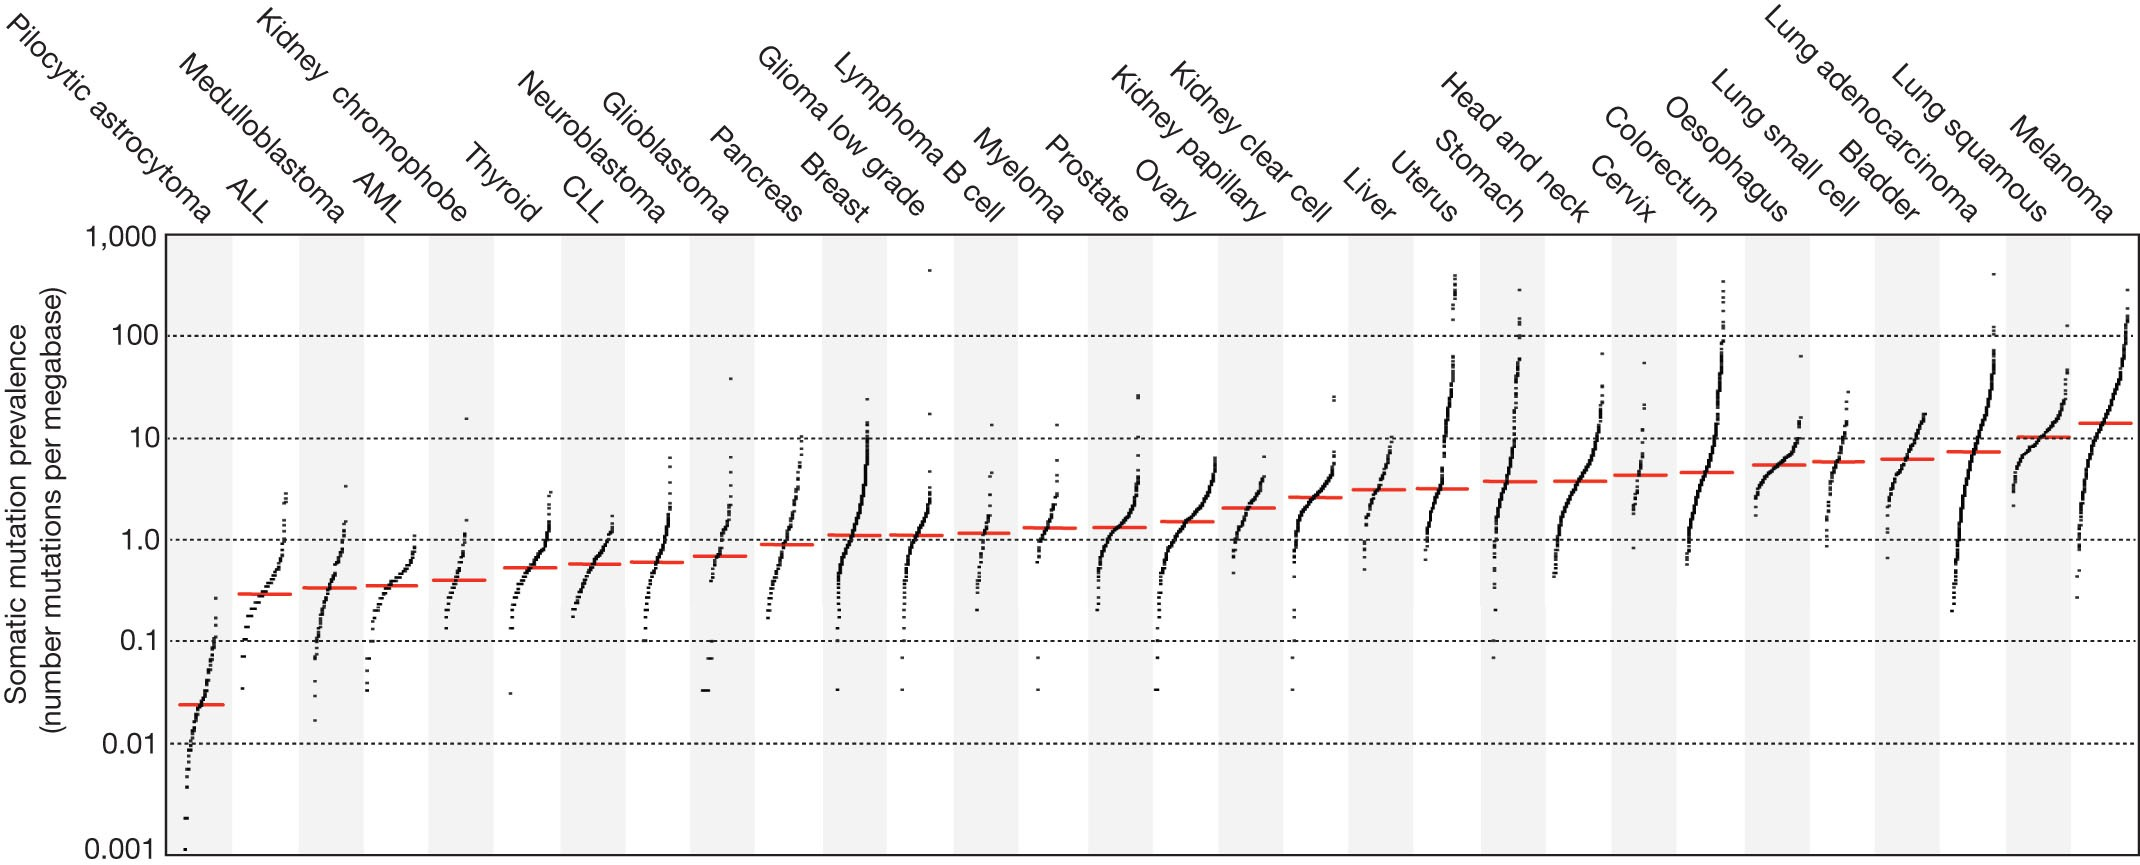
\includegraphics[width=0.9\textwidth,height=0.9\textheight,keepaspectratio]{Sections/Lit_review/Resources/mut_sig_cancers.jpg}
    \caption{Image from \cite{Alexandrov2013-gi} showing the somatic mutations across the different human cancer. Each sample is represented by a dot and the red line is the median number of mutation in that tumour type. The y-axis is the number of mutations per megabases, and the cancer types are ordered by the median mutation count, which makes bladder cancer the 4th highest mutated cancer.}
    \label{fig:lit:cancer_mut_sig}
\end{figure}

\begin{figure}[!htb]    
    \centering
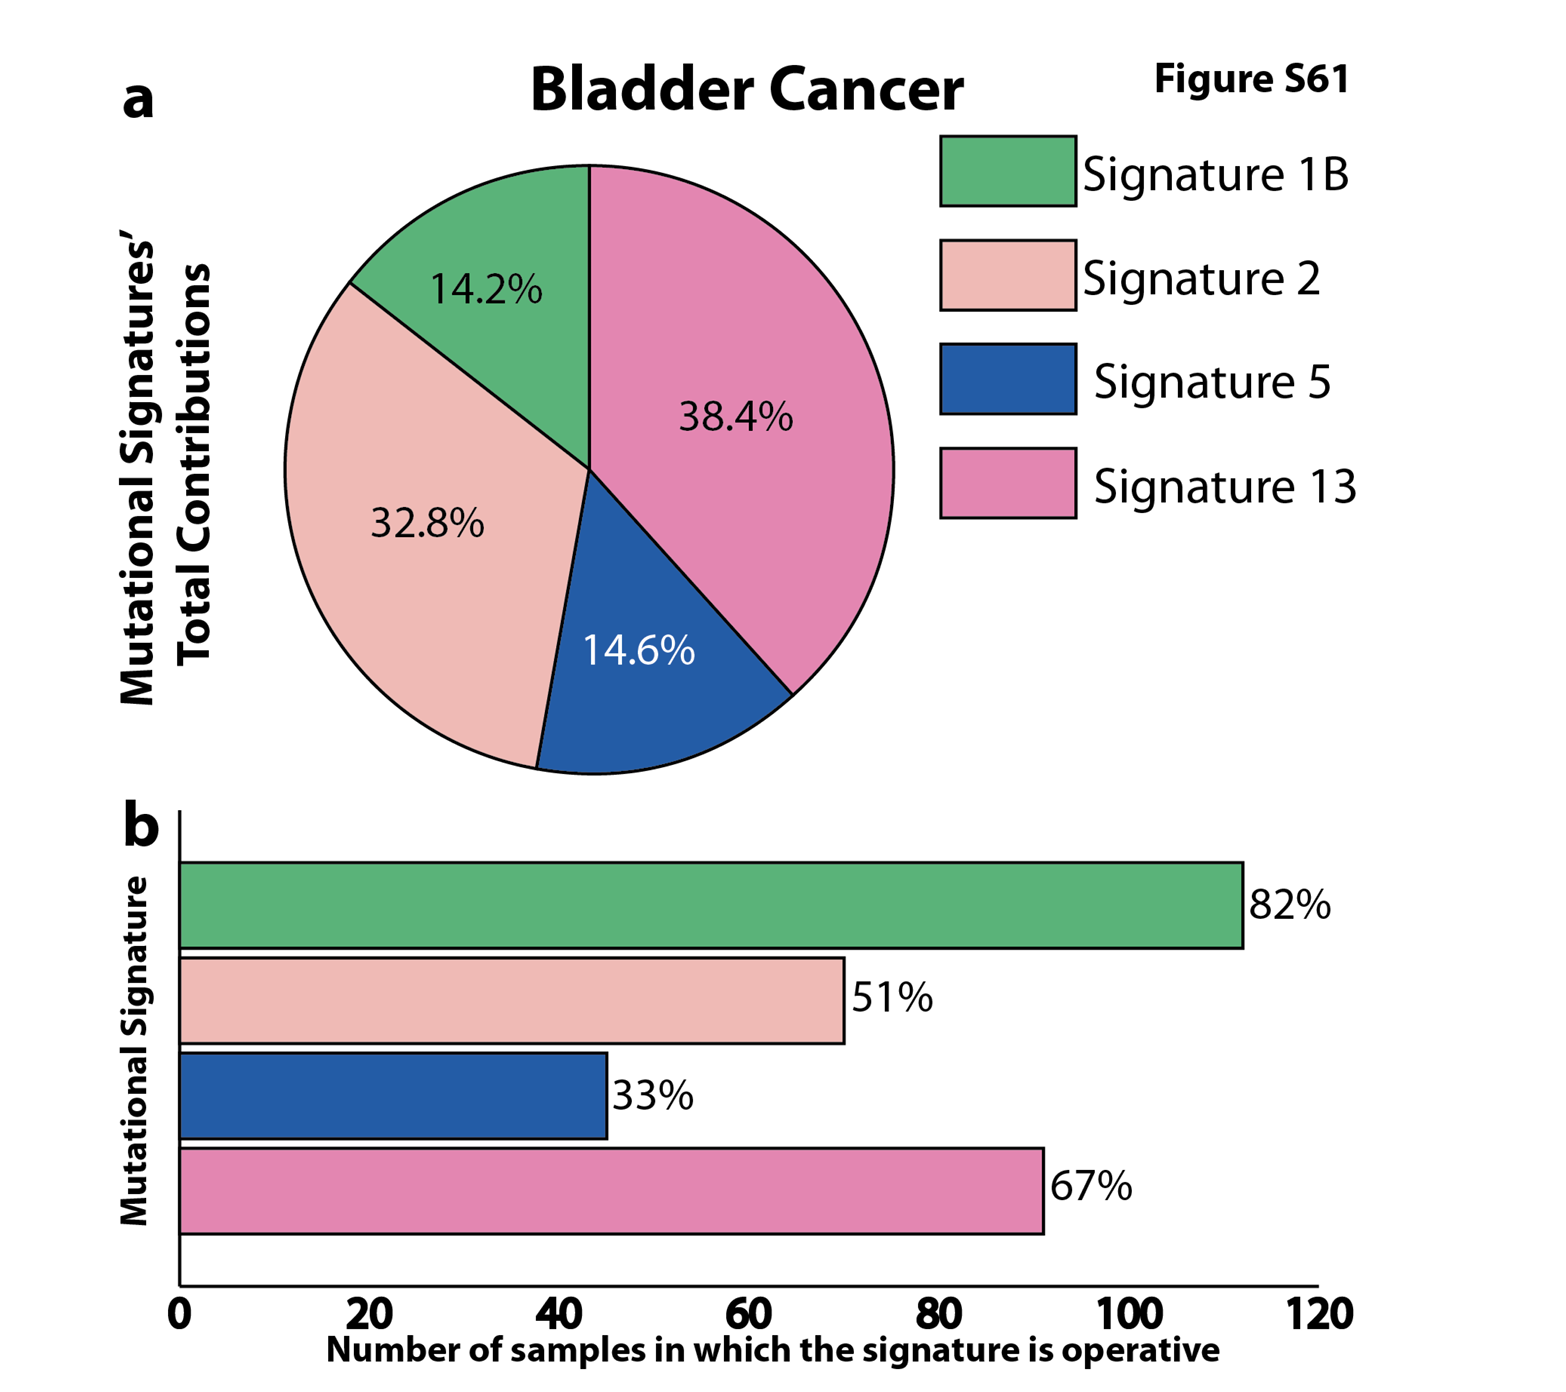
\includegraphics[width=0.6\textwidth,height=0.6\textheight,keepaspectratio]{Sections/Lit_review/Resources/bladder_mut_sig.png}
    \caption{Image from Supplementary \cite{Alexandrov2013-gi} showing the mutation signatures for bladder cancer. a) showing the the contribution of each signature while b) the number of samples where it was found. }
    \label{fig:lit:bladder_mut_sig}
\end{figure}


% epigenetic burden
The high somatic mutation burden is also highlighted by other research \cite{Tcga2014-dr, Robertson2017-mg, Kamoun2020-tj}. The first two studies found that the mutations disrupt the epigenetic machinery. Understanding these anomalies have the potential to lead to new potential targeted treatments.



\pagebreak

\begin{todolist}
    \item Overview of the bladder cancer 
    \begin{todolist}
        \item [\done] Statistics worlwide/UK/Europe
        \item [\done] Main causes, metal contamination
        \item [\done] More prevalent in men
        \item NMIBC vs MIBC
    \end{todolist}
    \item Why it is so bad? 
    \begin{todolist}
        \item [\done] Impact of the quality of life, treatment cost?
        \item Metastasis sites
    \end{todolist}
    \item Efforts to solve it and introduce the subtypes problem
    \item Introduce the consensus, TCGA and Lund
    \begin{todolist}
        \item Table markers for Consensus
        \item Table markers for TCGA
        \item Table markers for Lund
        \item Mutations found and relevant
    \end{todolist}
    \item Talk about the current UK trial that is using TCGA subtypes, stressing the importance of finding the right subgroups
    \item Healthy dataset 
    \begin{todolist}
        \item different tissue types
        \item what are the sources of the dataset
        \item gene markers for each dataset
    \end{todolist}

\end{todolist}

\subsection{Tissue types of bladder cancer?}

\subsubsection{TCGA}


% Cover the Data in TCGA

% RNA-seq data

% Mutations

% Copy Number variation

% What type of tissue samples were used, more aggresive tumours

% How long did the study lasted, some of the relevant publications

\subsubsection{Consensus}

\subsubsection{Lund}

% How did they combined the different datasets


\subsection{Non-cancerous dataset}

% What are the three different types of tissues used?

% From which datasets where those used? Bladder vs Uropathies

% Properties of P0, Abs-Ca and Undifferentiated. Why it is important to include all of this? Abs-Ca related more to Luminal and Undiff more to Basal

\subsection{Conclusion}

% Talk about the